% PDF output (no extra blank pages, equal margins)
% \documentclass[a4paper,12pt,openright]{report}
% Two-sided printing binding (extra blank pages in order to start chapters on the right)
% This option requires uncommenting the selected lines in this document
\documentclass[a4paper,twoside,12pt,openright]{report}

% PAGE CONFIGURATION

\usepackage{parskip}                              % no indent
\usepackage{setspace}                             % line spacing, we'll use \setstretch{1.2}
\usepackage[a4paper, bottom=3cm]{geometry}        % margins
\usepackage{fancyhdr}                             % head and foot
    \pagestyle{fancy}                                 % set page to use it
    \fancyhf{}                                        % fancyhdr setup
    \fancyhead[L]{{\scshape\nouppercase\leftmark}}    % small caps chapter name in the header
    \fancyhead[R]{\thepage}                           % page number top right
    % \fancyfoot[C]{\emph{DRAFT Printed on \today}}     % foot
    \renewcommand{\headrulewidth}{0.4pt}              % header line
    \setlength{\headheight}{14.5pt}                   % header setup


% BIBLIOGRAPHY

\usepackage[backend=biber, style=authoryear]{biblatex}    % biblatex instead of bibtex
% \newcommand*{\bibtitle}{References}
    \renewcommand*{\bibfont}{\raggedright\small}              % smaller and left-aligned


% TEXT

\usepackage[T1]{fontenc}                        % letters such as ç, ò, etc
% \usepackage{mlmodern}                           % thicker computer modern font
\usepackage{mathpazo}                           % change font to palatino
\usepackage{mathtools,amsmath,amssymb,amsthm}   % math symbols, and theorems
\usepackage{dsfont}                             % indicator function
\usepackage{siunitx}                            % writing units (15 h, 10 kg, etc)


% TEXT FORMATTING

\usepackage[scaled]{helvet}                       % font for titles
% \setcounter{secnumdepth}{n}                       % no numbers in {n*sub}sections
% \numberwithin{equation}{chapter}                  % equation numbering
\usepackage{sectsty}                              % custimise section fonts
    \allsectionsfont{\sffamily}                       % set font for all sections
\usepackage[dvipsnames]{xcolor}                   % colors for the hyperlinks
% \definecolor{purplecite}{RGB}{202, 97, 228}         % define new color
\usepackage{enumitem}                             % fancy enumerate: nested lists and more
\usepackage{pifont}                               % extra bullet poins
    \renewcommand{\labelitemi}{\ding{109}}            % change default itemize
\usepackage{hyperref}                             % clickable hyperlinks
    \hypersetup{                                      % colored hyperlinks
        colorlinks = true,
        % filecolor = magenta,
        linkcolor = NavyBlue,
        % linkcolor= black,
        urlcolor = blue,
        citecolor = JungleGreen,
    }


% FIGURES

\usepackage{graphicx}                                         % include figures
\usepackage{pdfpages}                                         % insert pdf page \includepdf{}
\usepackage{pgfplots}                                         % plotting directly to latex
    \pgfplotsset{compat=1.18}                                     % compatibility settings for pgfplots
\usepackage{xltabular}                                        % long table with adaptative widths
\usepackage{subcaption}                                       % subfigures
\usepackage[format=plain,justification=centering]{caption}    % custom captions
    \captionsetup{font=small}                                     % caption package setup


% DRAFT

\usepackage{lipsum}                                     % lorem ipsum
\usepackage[color=pink]{todonotes}                      % to-do notes \todo{}
    \setlength{\marginparwidth}{2.3cm}                      % set margin for the notes
    \newcommand{\tocite}[1]{\todo[color=yellow]{#1}}        % custom to-do environment
\usepackage{tcolorbox}                                  % create boxes
    \newtcolorbox{redbox}{                                  % red box environment \begin{redbox}
      colframe=red!50,
      colback=red!10,
      boxrule=0.3mm,
      arc=0mm
    }
\newcommand {\Z}{\mathbb{Z}}                    % shortcuts for symbols
\newcommand {\R}{\mathbb{R}}
\newcommand {\diff}{\mathrm{d}}

\newtheorem{theorem}{Theorem}                   % theorem environments
\newtheorem{definition}{Definition}
\newtheorem{proposition}{Proposition}
\newtheorem*{proposition*}{Proposition}
\newtheorem{lemma}{Lemma}
\newtheorem{remark}{Remark}
\newtheorem{corollary}{Corollary}
\newtheorem{example}{Example}
\newtheorem{codedef}{Code}
\newtheorem{program}{Program}
\newtheorem{notation}{Notation}

\newcommand{\code}[1]{\texttt{#1}}              % monospace text for code

% \newenvironment{greyproof}[1][\proofname]{    % grey proofs
%   \proof[#1]
%   \color{darkgray}
% }{
%   \endproof
% }

\addbibresource{preamble/references.bib}

\hypersetup{                            % uncomment to print
    colorlinks = true,
    % filecolor = magenta,
    % linkcolor = NavyBlue,
    linkcolor= black,
    urlcolor = blue,
    citecolor = NavyBlue,
}

\date{September 2024}

\begin{document}

% \shipout\null         % to include uncounted blank pages

\pagenumbering{roman}
\singlespacing

% printed version assumes this to be disabled:
% \includepdf{preamble/cover.pdf}   % to include a pdf cover
\thispagestyle{empty}

\begin{titlepage}
    \newgeometry{margin=1in, top=2in, bottom=2in} % Custom margins for title page
    \begin{center}
        \Large Universitat d'Exemple\\[0.2em]
        \LARGE Facultat d'Exemple i Exemple
    \end{center}
    \vspace{3cm}
    \begin{center}
        \large Master in Exampled Examples and Examples of Examples\\[0.2em]
        \LARGE\scshape Master's thesis
    \end{center}
    \vspace{1cm}
    \begin{center}
        {\color{RoyalBlue}\Huge\bf Title first line\\[0.5em]
        title second line}\\[1.5em]
        {\LARGE\bf Víctor Villegas-Morral}
    \end{center}
    \vspace{3cm}
    \begin{center}
        \Large Supervised by Supervisor \\[0.5em]
        \large Month YYYY
    \end{center}
    % \vspace{1cm}
    \begin{figure}[b]
        \centering
        \begin{subfigure}{0.62\textwidth}
            \centering
            
\includegraphics[height=4.8em]{figures/cover-logo-1.jpeg}
        \end{subfigure}
        \hfill
        \begin{subfigure}{0.36\textwidth}
            \centering
            
\includegraphics[height=4.8em]{figures/cover-logo-2.jpeg}
        \end{subfigure}
    \end{figure}
    \restoregeometry
\end{titlepage}

\thispagestyle{empty}\null              % uncomment to print

\thispagestyle{plain}                                   % simple page numbering
\newgeometry{margin=4.25cm, bottom=3cm, top=3cm}        % should be the same as in the abstract
\setstretch{1.2}

\null           % null character necessary to add vertical space at the beginning of the page
\vspace{5cm}

\begin{center}
    {\Large\bfseries\sffamily  Acknowledgements}
\end{center}

\vspace{0.5em}

\lipsum[1]

\restoregeometry
\thispagestyle{empty}\null              % uncomment to print
\thispagestyle{plain}                                   % simple page numbering
\newgeometry{margin=4.25cm, bottom=3cm, top=3cm}        % should be the same as in the acknowledgements
\setstretch{1.2}

\begin{center}
    {\Large\bfseries\sffamily  Abstract}
\end{center}

\vspace{0.5em}

In English.

\lipsum[1]

\vspace{2em}

\begin{center}
    {\Large\bfseries\sffamily Resum}
\end{center}

\vspace{0.5em}

En català.

\lipsum[1]

\restoregeometry

\setstretch{1.2}    % line spacing

\thispagestyle{empty}\null              % uncomment to print
\tableofcontents
\newpage

% (print) add another one if necessary. sections must start on the right.
\thispagestyle{empty}\null\newpage      % uncomment to print

\pagenumbering{arabic} 
\setcounter{page}{1}

\chapter*{Nomenclature}\label{ch:nomenclature}
\addcontentsline{toc}{chapter}{Nomenclature}
\markboth{Nomenclature}{}

%% It can be done with the nomencl package too.
% -----------------------------------------------------
% \usepackage[intoc]{nomencl} % nomenclature in ToC
% \makenomenclature
% \renewcommand{\nomname}{Symbols and Definitions}
% \renewcommand{\nompreamble}{This section provides a reference for the notation used throughout the project. \vspace{2em}}
% \setlength{\nomlabelwidth}{4em}
% -----------------------------------------------------

This section serves as a reference for the notation used throughout the text.
\vspace{1em}

\renewcommand{\arraystretch}{1.2}

{\small                                 % smaller font size for the table
\begin{xltabular}{\textwidth}{ 
    >{\centering\arraybackslash}p{0.12\textwidth}   % first column: 12% of text width
    >{\centering\arraybackslash}p{0.2\textwidth}
    X                                               % third column: take up the remaining space
    >{\centering\arraybackslash}p{0.11\textwidth}   % fourth column: 11% of text width
}
    \hline
    \textbf{Symbol} & \textbf{Code} & \multicolumn{1}{c}{\textbf{Description}} & \textbf{Value} \\      % header
    \hline
        $T_0$ & \code{t0} & Typical time scale & \SI{2}{\hour} \\
        $R_0$ & \code{r0} & Typical length scale & \SI{5}{\micro\meter} \\
    \hline
\end{xltabular}
}








% (print) add another one if necessary. sections must start on the right.
\thispagestyle{empty}\null\newpage      % uncomment to print

\chapter{Introduction}
\markboth{Introduction}{}

This is the introduction \parencite{vm_2024}. The colour for each type of hyperlink can be tuned.


\section{Cites and references}

As seen in \cite{vm_2024}, the colour orange is a mix of red and yellow (see Figure \ref{fig:orange}). 

\begin{figure}[htbp]      % preferences in order: [h]ere, [t]op, [b]ottom, [p]age
    \centering
    
\includegraphics[width=0.3\textwidth]{figures/orange.jpeg}
    \caption{Orange. Adapted from \cite{vm_2024}.}
    \label{fig:orange}
\end{figure}

All the code developed for this project is available on my \href{https://github.com/villegas-morral/}{personal GitHub} \footnote{https://github.com/villegas-morral/}. See the colour orange in Figure \ref{fig:orange}.


\section{Text}

\lipsum[3]
% the name in brackets is the one used in the contents
\chapter[A chapter with long title]{A chapter with a very long \\ title that wouldn't fit}\label{ch:2-abm}
\markboth{Name of the chapter in the header}{}

This document uses Helvetica for the section and chapter titles, and Palatino for the text and equations (see \code{packages.tex}). Font size is set to 12pt, and line spacing to 1.2pt.



\section{The first section}


\subsection{The first subsection}

\begin{proposition}\label{prop:example}
    Definitions, propositions, and more theorem environments are defined in \code{macros.tex}.
    \begin{itemize}
        \item The default bullet point for \code{itemize} is changed to this one.
        \item Code is written using the command \code{\textbackslash code\{\}}.
    \end{itemize}
\end{proposition}

We can plot functions using \LaTeX, as shown in Figure \ref{fig:example-function}.

\begin{figure}[htp]
    \centering
    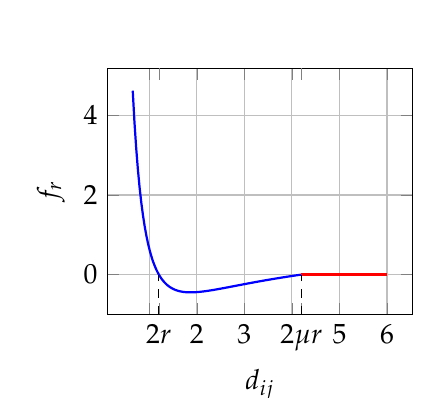
\begin{tikzpicture}
        \begin{axis}[
            width=0.45\textwidth,
            xlabel={$d_{ij}$}, 
            ylabel={$f_r$},
            % title={title}
            grid=both,
            domain=0:6,
            samples=100, 
            ymin=-1,
            xtick={1, 2, 3, 4, 5, 6},
            xticklabels={,2,3,,5,6}, 
            extra x ticks={1.2, 4.2}, 
            extra x tick labels={$2r$, $2\mu r$},
            extra x tick style={grid=none}
        ]
            \addplot[domain=0.65:4.2, samples=100, thick, color=blue] {(2*0.6/x - 1)*(2*.6*3.5/x - 1)};
            \addplot[domain=4.2:6, samples=100, thick, color=red] {0};

            \addplot[dashed, thin, black] coordinates {(1.2, -1) (1.2, 0)};
            \addplot[dashed, thin, black] coordinates {(4.2, -1) (4.2, 0)};
        \end{axis}
    \end{tikzpicture}    
    \caption{Example function $f_r$.}
    \label{fig:example-function}
\end{figure}

Recall that the example function $f_r$ is given by the following expression,
\begin{equation}\label{eq:example-function}
    f_r=
    \begin{dcases}
        \frac{a}{b}\alpha_\text{sub} &\quad \text{if $a<c$} \\
        ab\sqrt{a+c} &\quad \text{if $a\geq c$} \\
        0 &\quad \text{otherwise.}
    \end{dcases}
\end{equation}


\subsection{The second subsection}

Nesting in \code{enumerate}:

\begin{enumerate}
    \item First.
    \begin{enumerate}[label=\roman*.] % [label=\theenumi.\arabic*.]
        \item First first.
        \item Second first.
    \end{enumerate}
    \item Second.
\end{enumerate}

We can recall an equation while keeping the numbering. If there is a space between the text and the text and the \code{equation} environment, the space between these will increase because the equation will be assumed to be a separate paragraph. Keep this in mind to ensure consistency.
\begin{equation}\tag{\ref{eq:example-function}}
    f_r=
    \begin{dcases}
        \frac{a}{b}\alpha_\text{sub} &\quad \text{if $a<c$} \\
        ab\sqrt{a+c} &\quad \text{if $a\geq c$} \\
        0 &\quad \text{otherwise.}
    \end{dcases}
\end{equation}

If there is a space between the text and the text and the \code{equation} environment, the space between these will increase because the equation will be assumed to be a separate paragraph. Keep this in mind to ensure consistency.

\begin{equation}\tag{\ref{eq:example-function}}
    f_r=
    \begin{dcases}
        \frac{a}{b}\alpha_\text{sub} &\quad \text{if $a<c$} \\
        ab\sqrt{a+c} &\quad \text{if $a\geq c$} \\
        0 &\quad \text{otherwise.}
    \end{dcases}
\end{equation}

\begin{redbox}
    This is a custom environment for red boxes.
\end{redbox}

We can also\todo{like this} use margin notes. \tocite{like this}
\chapter{Conclusions and further work}
% \addcontentsline{toc}{chapter}{Conclusions}
\markboth{Conclusions and further work}{}

\lipsum[1-2]
\chapter*{Appendix}\label{ch:appendix}
\addcontentsline{toc}{chapter}{Appendix}
\renewcommand{\thesection}{A.\arabic{section}}


\section{First appendix section}

Note that in the appendix the numbering of sections uses an A.



\section{First appendix section}

\begin{proposition*}[Proposition \ref{prop:example}]
    We can create unnumbered propositions and add titles in brackets.
\end{proposition*}

\begin{proof}
    This is an example of a proof.
\end{proof}

% \clearpage
% \addcontentsline{toc}{chapter}{References}
\printbibliography[title={References}, heading=bibintoc]

\end{document}
